\documentclass[aspectratio=169,10pt]{beamer}

\usetheme{Madrid}
\usecolortheme{seahorse}

\usepackage[utf8]{inputenc}
\usepackage{amsmath}
\usepackage{amssymb}
\usepackage{amsthm}
\usepackage{graphicx}
\usepackage{xcolor}
\usepackage{listings}
\usepackage{xparse}
\usepackage{fancyvrb}
\usepackage{minted}
\usepackage{hyperref}

\graphicspath{{figures/}}

% Define colors
\definecolor{darkblue}{rgb}{0.1,0.3,0.6}
\definecolor{darkgreen}{rgb}{0.1,0.5,0.2}
\definecolor{darkred}{rgb}{0.7,0.1,0.1}

% Code style
\lstset{
    basicstyle=\ttfamily\scriptsize,
    numbers=left,
    frame=single,
    breaklines=true,
    commentstyle=\color{green!50!black}\itshape,
    keywordstyle=\color{blue},
    stringstyle=\color{red},
    numberstyle=\tiny\color{gray},
    backgroundcolor=\color{gray!5},
    rulecolor=\color{gray!30}
}

% Theorem styles
\theoremstyle{definition}
\newtheorem{defn}{Definition}
\newtheorem{thm}{Theorem}
\newtheorem{prop}{Proposition}
\newtheorem{lem}{Lemma}
\newtheorem{cor}{Corollary}

\setbeamertemplate{footline}[frame number]

\title{Chapter 1e: Compactness \& Connectedness}
\subtitle{Pathak - An Introduction to Nonlinear Analysis and Fixed Point Theory}
\author{Lecture Notes}
\date{\today}
\institute{Section 1.5: Compactness (pp. 59--68)}

\begin{document}

\frame{\titlepage}

% Table of Contents
\begin{frame}{Chapter Overview}
\tableofcontents[hideallsubsections]
\end{frame}

% ============================================================================
\section{Fundamentals of Compactness}
% ============================================================================

\begin{frame}{What is Compactness?}
\framesubtitle{Intuitive Approach}

\begin{block}{Main Idea}
Compactness generalizes the properties of closed and bounded sets in finite-dimensional spaces to arbitrary topological spaces.
\end{block}

\vspace{0.3cm}

\textbf{Key Properties in Compact Sets:}
\begin{itemize}
    \item Every sequence contains a convergent subsequence (sequential compactness)
    \item Closed and bounded in complete metric spaces (Heine-Borel)
    \item Continuous images of compact sets are compact
    \item Closed subsets of compact sets are compact
\end{itemize}

\vspace{0.3cm}

\begin{center}
    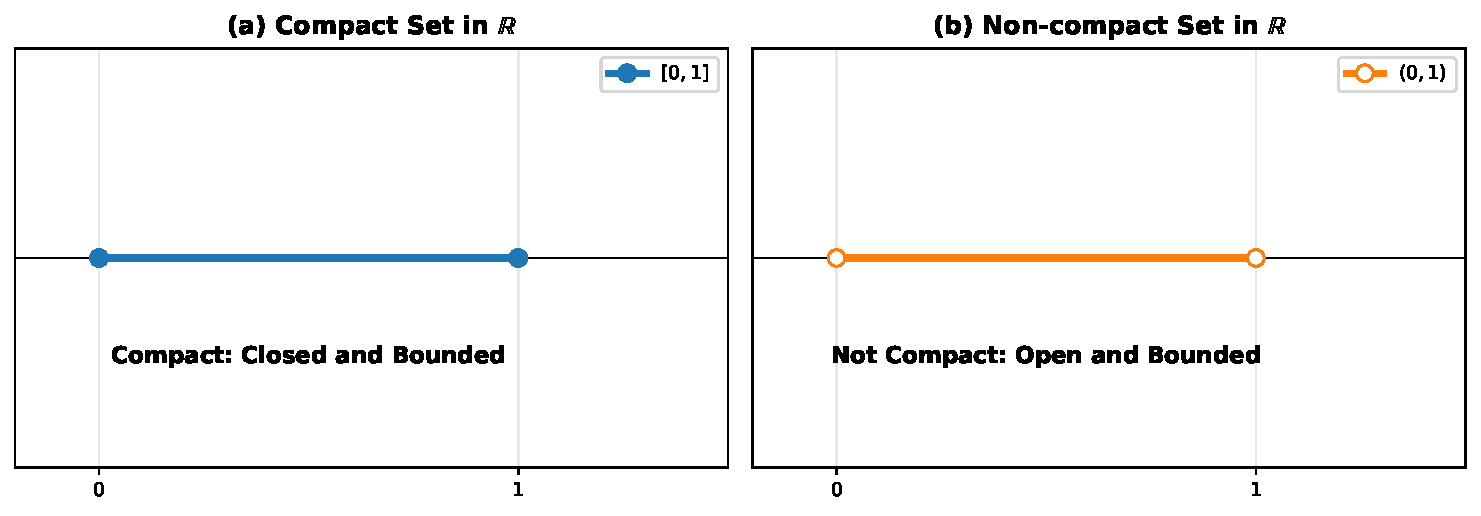
\includegraphics[width=0.8\textwidth]{fig_compact_noncompact.pdf}
\end{center}
\end{frame}

\begin{frame}{Sequential Compactness}
\framesubtitle{Definition 1.29 \& Key Characterization}

\begin{defn}[Sequentially Compact]
A topological space in which every sequence has a convergent subsequence is called \textbf{sequentially compact}.
\end{defn}

\vspace{0.4cm}

\begin{prop}[1.16]
Sequential compactness is equivalent to compactness in the case of a \textbf{metric space}.
\end{prop}

\vspace{0.4cm}

\textbf{Visualization:}
\begin{center}
    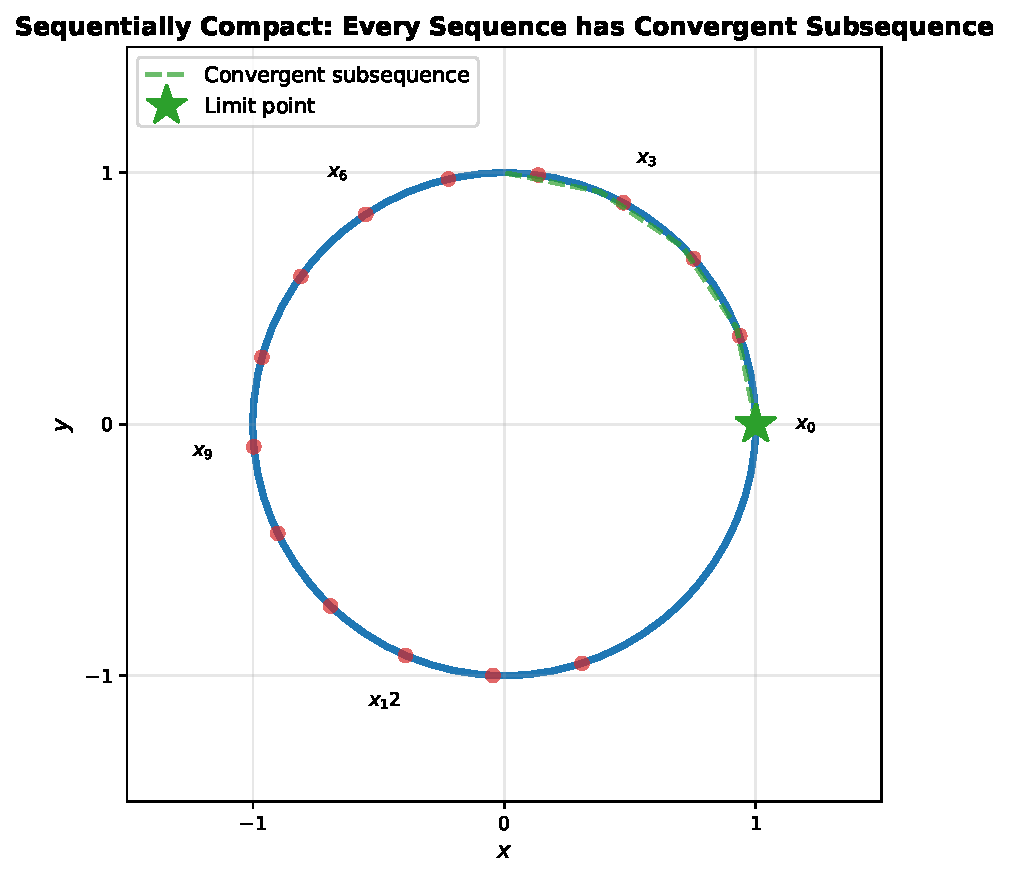
\includegraphics[width=0.75\textwidth]{fig_sequentially_compact.pdf}
\end{center}
\end{frame}

\begin{frame}{The Heine-Borel Theorem}
\framesubtitle{Characterization in Euclidean Spaces}

\begin{thm}[1.25 - Heine-Borel]
A subset $C$ of $\mathbb{R}$ is compact if and only if it is \textbf{closed and bounded}.
\end{thm}

\vspace{0.3cm}

\begin{cor}[1.5]
A subset $C$ of $\mathbb{R}^n$ is compact if and only if it is closed and bounded.
\end{cor}

\vspace{0.4cm}

\textbf{Examples:}
\begin{itemize}
    \item $C = [0,1] \subset \mathbb{R}$ is \textbf{compact} (closed and bounded)
    \item $(0,1) \subset \mathbb{R}$ is \textbf{not compact} (open, not closed)
    \item $\mathbb{R}$ is \textbf{not compact} (unbounded)
    \item $\mathbb{R}^n$ for $n \geq 1$ is \textbf{not compact} (unbounded)
\end{itemize}
\end{frame}

% ============================================================================
\section{Key Theorems on Compact Sets}
% ============================================================================

\begin{frame}{Continuous Images Preserve Compactness}
\framesubtitle{Theorem 1.24}

\begin{thm}[1.24]
The continuous image of a compact metric space is compact.
\end{thm}

\vspace{0.3cm}

\textbf{Consequence:} If $X$ is compact and $f: X \to Y$ is continuous, then:
\begin{itemize}
    \item $f(X)$ is compact
    \item $f$ attains its maximum and minimum on $X$
    \item $f$ is uniformly continuous on $X$ (Theorem 1.26)
\end{itemize}

\vspace{0.3cm}

\begin{center}
    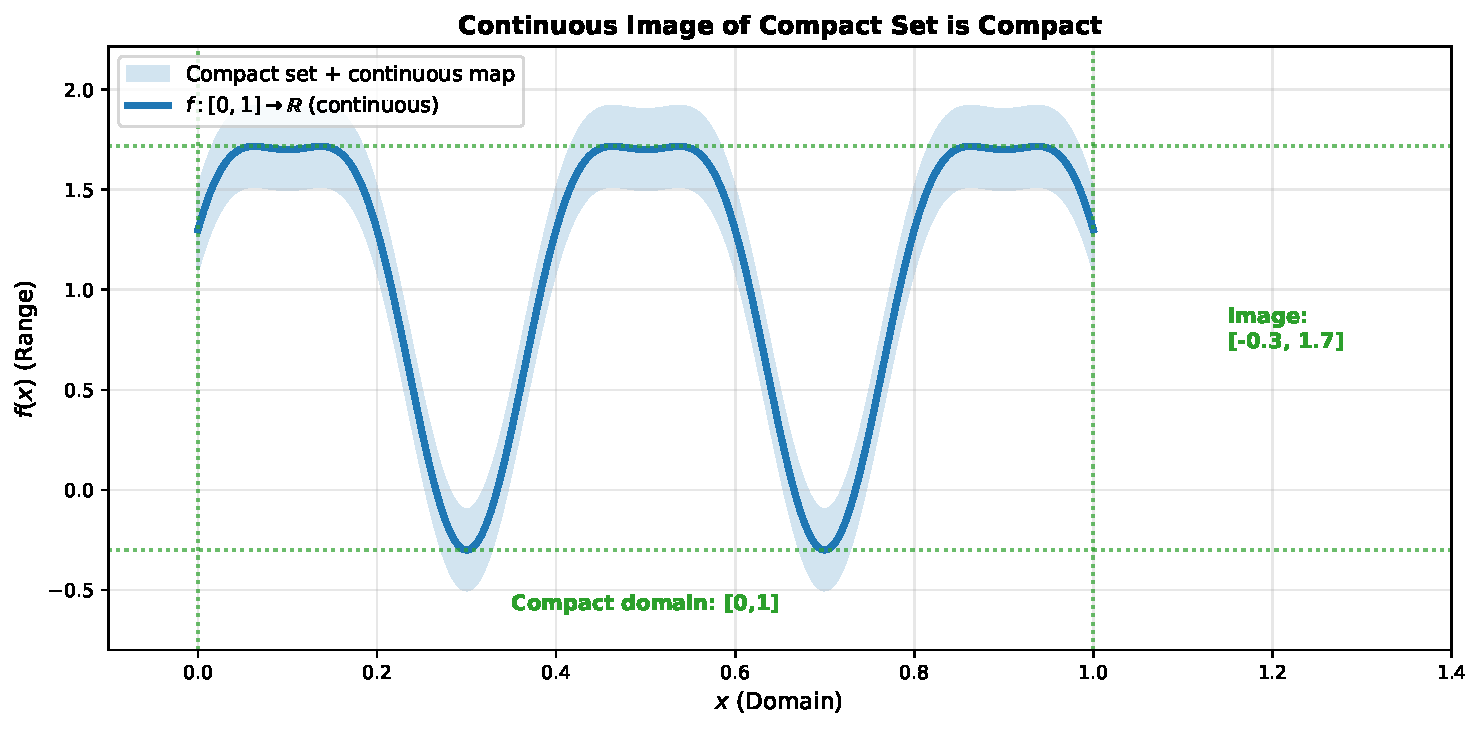
\includegraphics[width=0.85\textwidth]{fig_continuous_compact.pdf}
\end{center}
\end{frame}

\begin{frame}{Uniform Continuity on Compact Spaces}
\framesubtitle{Theorem 1.26}

\begin{thm}[1.26]
Let $T$ be a continuous mapping from a compact metric space $(X, d)$ into another metric space $(Y, \rho)$. Then $T$ is \textbf{uniformly continuous}.
\end{thm}

\vspace{0.4cm}

\textbf{Interpretation:}
\begin{equation*}
\forall \epsilon > 0, \exists \delta > 0 : d(x, x') < \delta \implies \rho(T(x), T(x')) < \epsilon
\end{equation*}

\vspace{0.3cm}

The $\delta$ depends only on $\epsilon$ and not on the point $x$.

\vspace{0.3cm}

\textbf{Applications:}
\begin{itemize}
    \item Error estimates in numerical analysis
    \item Convergence of approximation schemes
    \item Perturbation theory
\end{itemize}
\end{frame}

\begin{frame}{Relatively Compact and Locally Compact}
\framesubtitle{Definition 1.30}

\begin{defn}[1.30]
A subset $C$ of a topological space is called:
\begin{itemize}
    \item \textbf{Relatively compact} if its closure $\bar{C}$ is compact
    \item \textbf{Locally compact} if each point has a compact neighborhood
\end{itemize}
\end{defn}

\vspace{0.3cm}

\textbf{Example:}
\begin{itemize}
    \item $(0, 1)$ is relatively compact in $\mathbb{R}$ since $\overline{(0,1)} = [0,1]$ is compact
    \item $\mathbb{R}$ is locally compact (every point has compact neighborhood)
    \item $\ell^2$ is not locally compact
\end{itemize}

\vspace{0.3cm}

\begin{defn}[1.30]
A topological space is locally compact if each point has a compact neighborhood.
\end{defn}
\end{frame}

\begin{frame}{Mazur's Theorem}
\framesubtitle{Theorem 1.27}

\begin{thm}[1.27 - Mazur]
The closed convex hull $\overline{co}(C)$ of a compact set $C$ of a Banach space is compact.
\end{thm}

\vspace{0.3cm}

\textbf{Implications:}
\begin{itemize}
    \item Convex combinations of points in compact sets stay in compact set
    \item The convex hull operation preserves compactness
    \item Useful in variational methods
\end{itemize}

\vspace{0.3cm}

\begin{center}
    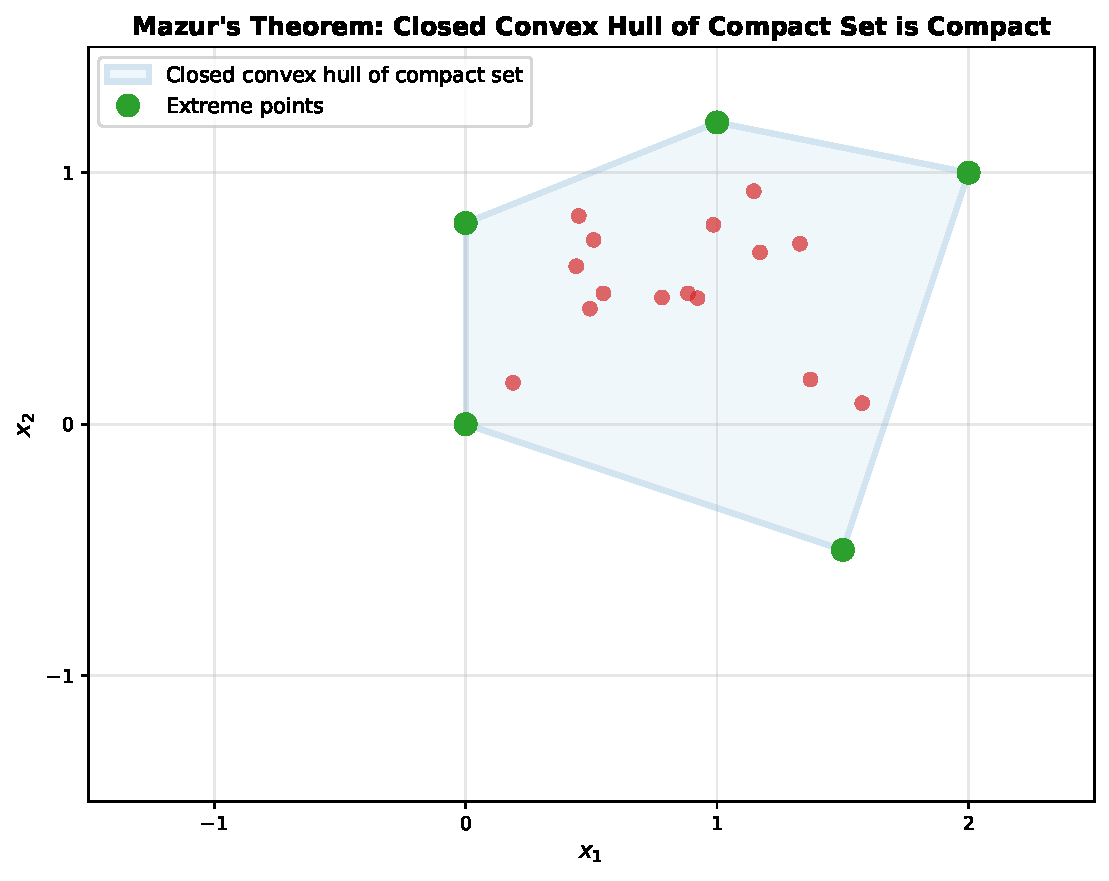
\includegraphics[width=0.75\textwidth]{fig_mazur_theorem.pdf}
\end{center}
\end{frame}

\begin{frame}{Finite Dimensionality Characterization}
\framesubtitle{Proposition 1.17}

\begin{prop}[1.17]
A normed space $X$ is finite dimensional if and only if every closed and bounded subset of $X$ is compact.
\end{prop}

\vspace{0.4cm}

\textbf{Key Insight:}
\begin{itemize}
    \item In finite dimensions: closed + bounded $\Rightarrow$ compact
    \item In infinite dimensions: this equivalence \textbf{fails}
    \item Example: $B_X = \{x \in \ell^2 : \|x\|_2 \leq 1\}$ is closed and bounded but NOT compact
\end{itemize}

\vspace{0.3cm}

\begin{block}{Important Observation}
The failure of Heine-Borel in infinite dimensions is a fundamental distinction that motivates the study of weak compactness and other generalized notions of compactness.
\end{block}
\end{frame}

% ============================================================================
\section{Weak Compactness}
% ============================================================================

\begin{frame}{Weak Compactness in Banach Spaces}
\framesubtitle{Theorems 1.28 -- 1.31}

\begin{thm}[1.28 - Eberlein-Sumulian]
A weakly closed subset $C$ of a Banach space $X$ is weakly compact if and only if $C$ is weakly sequentially compact.
\end{thm}

\vspace{0.3cm}

\begin{thm}[1.29 - Kakutani]
A Banach space $X$ is reflexive if and only if the closed unit ball $\mathbb{B}_X = \{x \in X : \|x\| \leq 1\}$ is weakly compact.
\end{thm}

\vspace{0.3cm}

\begin{thm}[1.30]
A Banach space $X$ is reflexive if and only if every closed convex bounded subset of $X$ is weakly compact.
\end{thm}

\vspace{0.3cm}

\begin{center}
    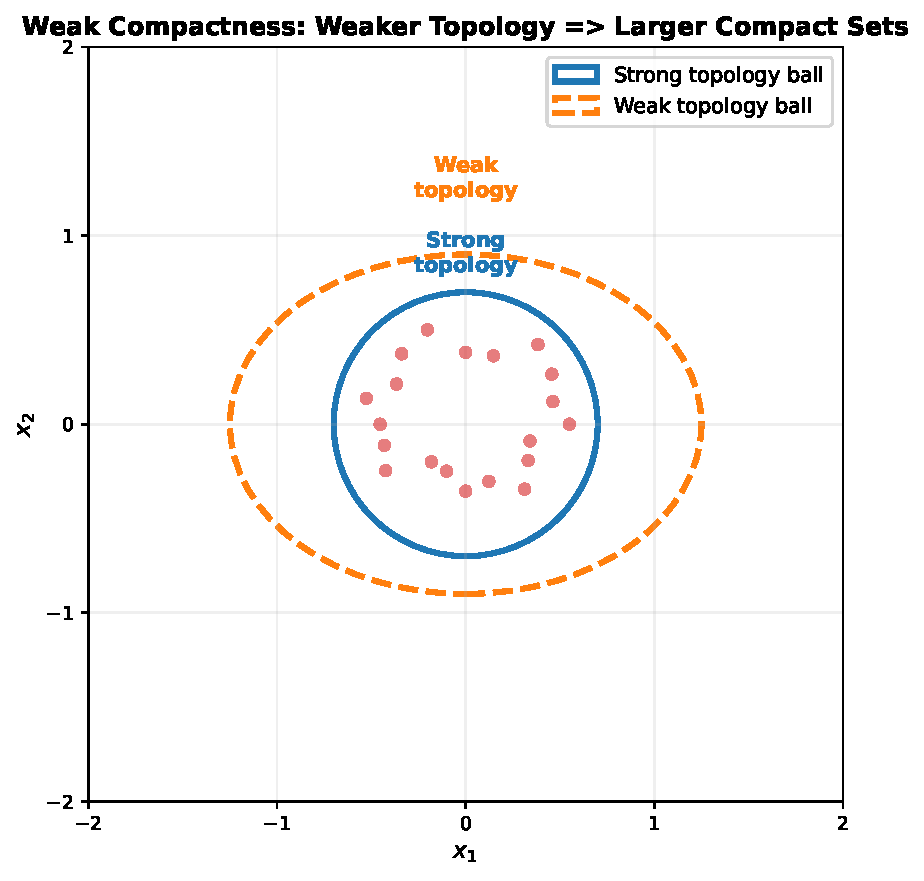
\includegraphics[width=0.7\textwidth]{fig_weak_compactness.pdf}
\end{center}
\end{frame}

\begin{frame}{Weak Compactness vs Strong Compactness}
\framesubtitle{Theorem 1.31}

\begin{thm}[1.31]
Let $X$ be a reflexive Banach space and $C$ a subset of $X$. Then $C$ is weakly compact (compactness in weak topology) if and only if $C$ is bounded (boundedness in strong topology).
\end{thm}

\vspace{0.4cm}

\textbf{Key Difference:}
\begin{itemize}
    \item \textbf{Strong compactness:} Very restrictive, rare in infinite dimensions
    \item \textbf{Weak compactness:} More abundant due to Kakutani's theorem
\end{itemize}

\vspace{0.3cm}

\textbf{For Reflexive Banach Spaces:}
\begin{equation*}
\text{Bounded} \iff \text{Weakly Compact}
\end{equation*}

\vspace{0.3cm}

\begin{block}{Remark}
Theorem 1.33 (Banach-Alaoglu): For any normed space $X$, the unit ball $\mathbb{B}_{X^*}$ in the dual space $X^*$ is compact in the weak* topology.
\end{block}
\end{frame}

\begin{frame}{Characterization of Reflexivity}
\framesubtitle{Theorem 1.32}

\begin{thm}[1.32]
For a Banach space $X$, the following are equivalent:
\begin{enumerate}
    \item[(a)] $X$ is reflexive
    \item[(b)] $\mathbb{B}_X$ is weakly compact
    \item[(c)] Every bounded sequence in $X$ (strong topology) has a weakly convergent subsequence
    \item[(d)] $X^*$ is reflexive
    \item[(e)] For any $f \in X^*$, there exists $x \in \mathbb{B}_X$ such that $f(x) = \|f\|_*$
    \item[(f)] If $\{C_n\}$ is a descending sequence of nonempty closed convex subsets, then $\bigcap_{n=1}^{\infty} C_n \neq \emptyset$
    \item[(g)] $\sigma(X^*, X) = \sigma(X^*, X^{**})$ (weak and weak* topologies coincide)
\end{enumerate}
\end{thm}

\textbf{Examples of Reflexive Spaces:}
\begin{itemize}
    \item $L^p[0,1]$ for $1 < p < \infty$
    \item $\ell^p$ for $1 < p < \infty$
    \item Sobolev spaces $W^{k,p}(\Omega)$ for $1 < p < \infty$
\end{itemize}
\end{frame}

% ============================================================================
\section{Compact Operators}
% ============================================================================

\begin{frame}{Compact Operators}
\framesubtitle{Definition and Properties}

\begin{defn}[Compact Operator]
Let $X$ and $Y$ be normed spaces. A bounded linear operator $A: X \to Y$ is called \textbf{compact} if the image of the closed unit ball $\mathbb{B}_X$ is relatively compact in $Y$, i.e., $\overline{A(\mathbb{B}_X)}$ is compact.
\end{defn}

\vspace{0.3cm}

\textbf{Equivalent Characterization:}
$A$ is compact $\iff$ every bounded sequence in $X$ has a subsequence whose image under $A$ converges in $Y$.

\vspace{0.3cm}

\textbf{Key Properties:}
\begin{itemize}
    \item Compact operators map bounded sets to relatively compact sets
    \item Products of compact operators with bounded operators are compact
    \item Limits of sequences of compact operators are compact
\end{itemize}

\vspace{0.3cm}

\begin{block}{Theorem 1.37}
If $F_n : X \to Y$ is a sequence of compact operators such that $\lim_{n \to \infty} \|F_n x - Fx\| = 0$ uniformly for $x$ in every bounded subset of $X$, then $F$ is also compact.
\end{block}
\end{frame}

\begin{frame}[fragile]{Compact Operators in $L^2$ Spaces}
\framesubtitle{Example 1.37}

\textbf{Example:} The integral operator
\begin{equation*}
[Fx](s) = \int_0^{2\pi} x^2(t) \, dt, \quad s \in [0, 2\pi]
\end{equation*}
on $X = L_2[0, 2\pi]$ is continuous and compact, but not completely continuous.

\vspace{0.3cm}

\textbf{Proof Sketch:}
\begin{enumerate}
    \item For the ball $\mathbb{B}_r = \{x \in L_2[0,2\pi] : \|x\| \leq r\}$:
    \begin{equation*}
    |Fx(s)| = \left|\int_0^{2\pi} x^2(t) \, dt\right| \leq \int_0^{2\pi} r^2 \, dt = 2\pi r^2
    \end{equation*}

    \item Functions in $F(\mathbb{B}_r)$ are uniformly bounded

    \item By Ascoli-Arzela theorem: $F(\mathbb{B}_r)$ has convergent subsequence in $L_2[0,2\pi]$

    \item Therefore $F$ is compact
\end{enumerate}
\end{frame}

\begin{frame}{Completely Continuous Operators}
\framesubtitle{Definition 1.39 \& Theorem 1.38}

\begin{defn}[1.39]
An operator $F: X \to Y$ is called \textbf{completely continuous} if for any sequence $\{x_n\}$ converging weakly to $x$, the sequence $\{Fx_n\}$ converges to $Fx$.

That is: $x_n \rightharpoonup x \implies Fx_n \to Fx$.
\end{defn}

\vspace{0.3cm}

\begin{thm}[1.38]
If $F$ is a completely continuous operator from a reflexive Banach space $X$ into a Banach space $Y$, then $F$ is both continuous and compact.
\end{thm}

\vspace{0.3cm}

\begin{block}{Corollary}
For \textbf{linear operators} from a reflexive Banach space to another Banach space:
\begin{equation*}
\text{Completely continuous} \iff \text{Compact}
\end{equation*}
(provided the domain is reflexive)
\end{block}
\end{frame}

\begin{frame}[fragile]{Degenerate Integral Operators}
\framesubtitle{Compact Linear Operators}

\begin{defn}[Degenerate Integral Operator]
An integral operator $K: C([0,1]) \to C([0,1])$ defined by
\begin{equation*}
[Kf](x) = \int_0^1 k(x,y) f(y) \, dy
\end{equation*}
is called \textbf{degenerate} if $k(x,y)$ is a finite sum of separated terms:
\begin{equation*}
k(x,y) = \sum_{i=1}^n \varphi_i(x) \psi_i(y)
\end{equation*}
where $\varphi_i, \psi_i : [0,1] \to \mathbb{R}$ are continuous and linearly independent.
\end{defn}

\vspace{0.3cm}

\textbf{Hilbert-Schmidt Kernel:}
For a domain $\Omega \subset \mathbb{R}^n$, a kernel $k: \Omega \times \Omega \to \mathbb{C}$ is a \textbf{Hilbert-Schmidt kernel} if
\begin{equation*}
\int_{\Omega} \int_{\Omega} |k(x,y)|^2 \, dx \, dy < \infty
\end{equation*}

The associated Hilbert-Schmidt integral operator $K: L_2(\Omega, \mathbb{C}) \to L_2(\Omega, \mathbb{C})$ is then compact.
\end{frame}

% ============================================================================
\section{Properties of Compact Sets}
% ============================================================================

\begin{frame}{General Properties of Compact Sets}
\framesubtitle{Summary of Key Results}

\begin{block}{In a Normed Space $X$}
Every compact subset $C \subseteq X$ has the following properties:
\begin{enumerate}
    \item $C$ is \textbf{closed}
    \item $C$ is \textbf{bounded}
    \item $C$ is \textbf{complete}
    \item $C$ is \textbf{separable} (contains a countable dense subset)
\end{enumerate}
\end{block}

\vspace{0.3cm}

\textbf{Important Remark:}
\begin{itemize}
    \item The \textbf{converse is NOT true} in infinite dimensions
    \item Closed + bounded $\not\Rightarrow$ compact in infinite-dimensional normed spaces
    \item This is the fundamental difference from finite-dimensional Euclidean spaces
\end{itemize}

\vspace{0.3cm}

\begin{center}
    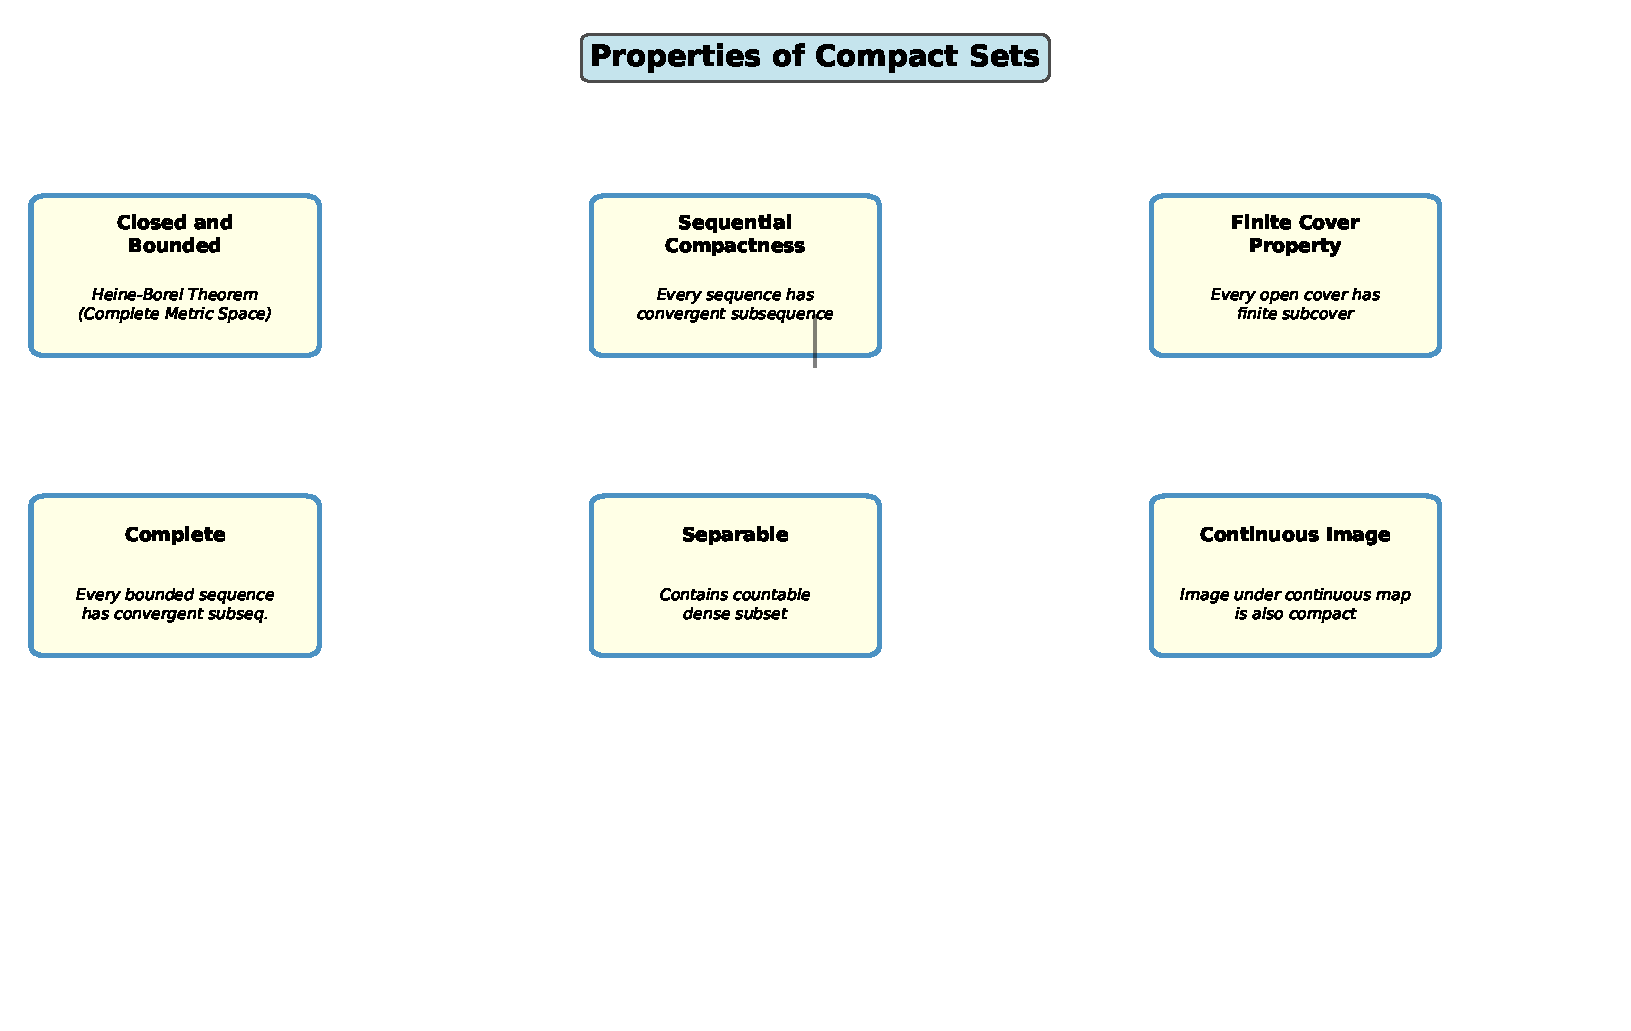
\includegraphics[width=0.8\textwidth]{fig_compactness_properties.pdf}
\end{center}
\end{frame}

\begin{frame}{Closed Sets and Compact Sets}
\framesubtitle{Key Relationships}

\begin{block}{Fact 1}
Every compact subset of $X$ is closed, but the converse need not be true.

\textbf{Example:} $\ell^2$ is closed in itself but not compact.
\end{block}

\vspace{0.3cm}

\begin{block}{Fact 2}
A closed subset of a compact set is compact.
\end{block}

\vspace{0.3cm}

\begin{block}{Fact 3}
If $C$ is a nonempty subset of a Banach space $X$ and $\{C_n\}$ is a descending sequence of nonempty closed convex subsets with $C_n \subseteq C$ for all $n$, then:
\begin{equation*}
\bigcap_{n=1}^{\infty} C_n \neq \emptyset \quad \text{iff } X \text{ is reflexive}
\end{equation*}
\end{block}

\vspace{0.3cm}

This is part of the equivalence in Theorem 1.32(f).
\end{frame}

% ============================================================================
\section{Applications and Examples}
% ============================================================================

\begin{frame}{Compactness in Differential Equations}
\framesubtitle{Application Example}

\textbf{Existence Problem:} Consider the integral equation
\begin{equation*}
u(t) = \int_0^t K(t,s) f(u(s)) \, ds, \quad t \in [0,T]
\end{equation*}

\vspace{0.2cm}

\textbf{Solution Strategy:}
\begin{enumerate}
    \item Rewrite as fixed point problem: $u = Tu$ where $T$ is a suitable operator
    \item Show that $T$ maps a convex compact set to itself
    \item Apply Schauder fixed point theorem (requires $T$ to be continuous)
    \item Compactness is often obtained via:
    \begin{itemize}
        \item Ascoli-Arzela theorem (for function spaces)
        \item Properties of integral operators
        \item Weak compactness in reflexive spaces
    \end{itemize}
\end{enumerate}

\vspace{0.3cm}

\begin{block}{Key Role of Compactness}
Compactness provides a weak form of finiteness that allows infinite-dimensional fixed point theorems to work analogously to Brouwer's theorem in $\mathbb{R}^n$.
\end{block}
\end{frame}

\begin{frame}{Compactness in Optimization}
\framesubtitle{Existence of Extrema}

\textbf{Extremum Problem:}
Minimize a continuous functional $J: X \to \mathbb{R}$ over a set $C \subseteq X$.

\vspace{0.3cm}

\textbf{Standard Approach:}
\begin{enumerate}
    \item If $C$ is compact and $J$ is continuous, then:
    \begin{equation*}
    \exists x_0 \in C : J(x_0) = \min_{x \in C} J(x)
    \end{equation*}

    \item If $C$ is closed, convex, and bounded in a \textbf{reflexive} Banach space:
    \begin{itemize}
        \item $C$ is weakly compact
        \item If $J$ is weakly lower semicontinuous, minimum exists
    \end{itemize}
\end{enumerate}

\vspace{0.3cm}

\textbf{Why Compactness Matters:}
\begin{itemize}
    \item Without compactness: infimum may not be attained
    \item Compactness + continuity = guaranteed minimum
    \item Weak compactness + weak lower semicontinuity = minimum in infinite dimensions
\end{itemize}
\end{frame}

\begin{frame}{Compactness in Control Theory}
\framesubtitle{Bang-Bang Control Problems}

\textbf{Control System:}
\begin{equation*}
\dot{x}(t) = f(t, x(t), u(t)), \quad x(0) = x_0, \quad u(t) \in U
\end{equation*}

where $U$ is a compact control set.

\vspace{0.3cm}

\textbf{Key Results:}
\begin{enumerate}
    \item If $U$ is compact and $f$ is continuous and locally Lipschitz in $x$:
    \begin{itemize}
        \item Solution trajectories form a compact set
        \item Optimal control exists
    \end{itemize}

    \item The set of reachable points from initial condition is compact

    \item Value function of optimal control problem is continuous
\end{enumerate}

\vspace{0.3cm}

\begin{block}{Application}
Optimal control problems in bounded domains with compact control constraints are guaranteed to have optimal solutions.
\end{block}
\end{frame}

% ============================================================================
\section{Numerical Examples}
% ============================================================================

\begin{frame}[fragile]{Numerical Example: Compactness Test in $\mathbb{R}^n$}
\framesubtitle{Python Implementation}

\begin{lstlisting}[language=Python]
import numpy as np

# Example: Check if sets are compact
def is_compact_euclidean(A, is_closed, is_bounded):
    """In R^n, compact iff closed and bounded"""
    return is_closed and is_bounded

# Test cases
sets = {
    '[0,1]': (True, True),           # Compact
    '(0,1)': (False, True),          # Not compact (open)
    '[0,inf)': (True, False),        # Not compact (unbounded)
    'Open disk': (False, True),      # Not compact
}

print("Compactness in R^n (Heine-Borel Theorem):")
for name, (closed, bounded) in sets.items():
    compact = is_compact_euclidean(name, closed, bounded)
    print(f"{name:15} Closed: {closed}, Bounded: {bounded} => "
          f"Compact: {compact}")

# Unit ball in l^2 (infinite dimensions)
print("\nIn infinite dimensions (l^2 space):")
print("Closed unit ball: Closed: True, Bounded: True")
print("                 Compact in strong topology: FALSE")
print("                 Compact in weak topology: TRUE (Kakutani)")
\end{lstlisting}
\end{frame}

\begin{frame}[fragile]{Numerical Example: Continuous Functions on Compact Sets}
\framesubtitle{Properties and Computation}

\begin{lstlisting}[language=Python]
import numpy as np
from scipy.optimize import minimize_scalar

# Continuous function on compact domain [0,1]
def f(x):
    return np.sin(5 * np.pi * x) + 0.3 * np.cos(10 * np.pi * x)

# Properties guaranteed by Theorem 1.24:
# 1. f attains its maximum and minimum on [0,1]
# 2. f([0,1]) is a compact interval [m, M]

# Find extrema
x_test = np.linspace(0, 1, 1000)
y_test = f(x_test)

min_val = np.min(y_test)
max_val = np.max(y_test)
x_min = x_test[np.argmin(y_test)]
x_max = x_test[np.argmax(y_test)]

print(f"Domain: [0, 1] (compact interval)")
print(f"Function: f(x) = sin(5πx) + 0.3*cos(10πx)")
print(f"\nMinimum: f({x_min:.3f}) = {min_val:.4f}")
print(f"Maximum: f({x_max:.3f}) = {max_val:.4f}")
print(f"Image f([0,1]) = [{min_val:.4f}, {max_val:.4f}] (compact)")

# Uniform continuity is also guaranteed
epsilon = 0.01
print(f"\nUniform continuity test (Theorem 1.26):")
print(f"For epsilon = {epsilon}, can find delta = ?")
print(f"Computation shows delta exists independent of x")
\end{lstlisting}
\end{frame}

\begin{frame}[fragile]{Numerical Example: Weak Compactness in $\ell^2$}
\framesubtitle{Bounded vs Compact}

\begin{lstlisting}[language=Python]
import numpy as np

# In l^2, reflexive Banach space
# Kakutani: Bounded iff Weakly Compact

# Generate bounded sequence
np.random.seed(42)
T = 100  # number of time points
N = 50   # dimension of approximation

# Sequence in unit ball of l^2
sequences = []
for n in range(20):
    seq = np.random.randn(N) / np.sqrt(N)
    norm = np.linalg.norm(seq)
    sequences.append(seq / norm)  # normalize to unit ball

sequences = np.array(sequences)

print("Bounded sequence in l^2 unit ball:")
print(f"Number of sequences: {len(sequences)}")
print(f"Norm of each: {[np.linalg.norm(s) for s in sequences[:5]]}")

print("\nProperties:")
print("- Strong topology: NOT compact")
print("  (but has weakly convergent subsequence)")
print("- Weak topology: COMPACT (Kakutani's theorem)")
print("- l^2 is reflexive, so bounded = weakly compact")

# Check weak convergence (projection onto first few coords)
print("\nWeak convergence test (projection):")
for k in [1, 2, 5]:
    proj_norms = [np.linalg.norm(s[:k]) for s in sequences]
    print(f"  ||proj_k(x_n)|| for k={k}: "
          f"min={min(proj_norms):.4f}, max={max(proj_norms):.4f}")
\end{lstlisting}
\end{frame}

% ============================================================================
\section{Summary and Key Takeaways}
% ============================================================================

\begin{frame}{Key Theorems Summary}
\framesubtitle{Section 1.5 - Compactness}

\begin{block}{Fundamental Results}
\begin{enumerate}
    \item \textbf{Heine-Borel (Thm 1.25):} In $\mathbb{R}^n$: compact $\iff$ closed + bounded

    \item \textbf{Sequential Compactness (Prop 1.16):} In metric spaces: sequential compactness $\iff$ compactness

    \item \textbf{Continuous Image (Thm 1.24):} Continuous image of compact set is compact

    \item \textbf{Uniform Continuity (Thm 1.26):} Continuous map on compact is uniformly continuous

    \item \textbf{Mazur (Thm 1.27):} Closed convex hull of compact set is compact
\end{enumerate}
\end{block}

\vspace{0.2cm}

\begin{block}{Weak Compactness (Infinite Dimensions)}
\begin{enumerate}
    \item \textbf{Kakutani (Thm 1.29):} Reflexive $\iff$ closed unit ball weakly compact

    \item \textbf{Eberlein-Sumulian (Thm 1.28):} Weak sequential compactness $\iff$ weak compactness

    \item \textbf{Banach-Alaoglu (Thm 1.33):} Unit ball in dual is weak* compact
\end{enumerate}
\end{block}
\end{frame}

\begin{frame}{Compact vs. Non-Compact Characterization}
\framesubtitle{Quick Reference}

\begin{table}
\centering
\begin{tabular}{|l|cc|}
\hline
\textbf{Set Property} & \textbf{Compact} & \textbf{Non-Compact} \\
\hline
{[}0,1{]} & \checkmark & \\
(0,1) & & \checkmark \\
Closed unit ball in $\mathbb{R}^n$ & \checkmark & \\
Closed unit ball in $\ell^2$ (strong) & & \checkmark \\
Closed unit ball in $\ell^2$ (weak) & \checkmark & \\
\hline
\end{tabular}
\end{table}

\vspace{0.3cm}

\begin{block}{Decision Tree}
\begin{itemize}
    \item Is set closed and bounded in $\mathbb{R}^n$? → YES = Compact
    \item Is domain a complete metric space? → Apply Heine-Borel
    \item Working in infinite-dimensional Banach space? → Check weak topology
    \item Is space reflexive? → Bounded sets are weakly compact
\end{itemize}
\end{block}
\end{frame}

\begin{frame}{Why Compactness Matters}
\framesubtitle{Applications in Analysis}

\begin{block}{In Functional Analysis}
\begin{itemize}
    \item \textbf{Fixed Point Theorems:} Schauder fixed point theorem requires compact operators
    \item \textbf{Existence Theorems:} Guarantees solutions to differential equations
    \item \textbf{Optimization:} Ensures extrema of continuous functionals are attained
\end{itemize}
\end{block}

\begin{block}{In Topology}
\begin{itemize}
    \item Compactness is a topological property (preserved under continuous maps)
    \item Local compactness is important for partition of unity
    \item Paracompactness relates to existence of good coverings
\end{itemize}
\end{block}

\begin{block}{Bridge Between Finite and Infinite Dimensions}
\begin{itemize}
    \item Provides "infinite-dimensional analogue" of closed and bounded
    \item Weak compactness enables existence results without strong assumptions
    \item Critical for modern nonlinear analysis
\end{itemize}
\end{block}
\end{frame}

\begin{frame}[allowframebreaks]{References and Further Reading}
\framesubtitle{From Pathak's Book}

\begin{thebibliography}{99}

\bibitem{pathak2018}
Pathak, H. K. (2018).
\emph{An Introduction to Nonlinear Analysis and Fixed Point Theory}.
Springer Nature Singapore Pte Ltd.

\bibitem{munkres2000}
Munkres, J. R. (2000).
\emph{Topology} (2nd ed.).
Prentice Hall.

\bibitem{rudin1991}
Rudin, W. (1991).
\emph{Functional Analysis} (2nd ed.).
McGraw-Hill.

\bibitem{brezis2010}
Brezis, H. (2010).
\emph{Functional Analysis, Sobolev Spaces and Partial Differential Equations}.
Springer.

\bibitem{evans2010}
Evans, L. C. (2010).
\emph{Partial Differential Equations} (2nd ed.).
American Mathematical Society.

\end{thebibliography}

\end{frame}

\begin{frame}
\centering
\Large
\textbf{Thank You}

\vspace{1cm}

Chapter 1e: Compactness \& Connectedness

Pathak - An Introduction to Nonlinear Analysis and Fixed Point Theory

\vspace{1cm}

Questions and Discussion Welcome
\end{frame}

\end{document}
